\documentclass[aps,letterpaper,10pt]{revtex4}

\usepackage{graphicx} % For images
\usepackage{float}    % For tables and other floats
\usepackage{verbatim} % For comments and other
\usepackage{amsmath}  % For math
\usepackage{amssymb}  % For more math
\usepackage{fullpage} % Set margins and place page numbers at bottom center
\usepackage{listings} % For source code
\usepackage{subfig}   % For subfigures
\usepackage[usenames,dvipsnames]{color} % For colors and names
\usepackage[pdftex]{hyperref}           % For hyperlinks and indexing the PDF
\usepackage[svgnames]{xcolor}
\usepackage{tikz}
\usetikzlibrary{arrows,shapes,positioning}
\tikzstyle arrowstyle=[scale=1]
\hypersetup{ % play with the different link colors here
    colorlinks,
    citecolor=blue,
    filecolor=blue,
    linkcolor=blue,
    urlcolor=blue % set to black to prevent printing blue links
}

\definecolor{mygrey}{gray}{.96} % Light Grey
\lstset{
	language=[ISO]C++,              % choose the language of the code ("language=Verilog" is popular as well)
   tabsize=3,							  % sets the size of the tabs in spaces (1 Tab is replaced with 3 spaces)
	basicstyle=\tiny,               % the size of the fonts that are used for the code
	numbers=left,                   % where to put the line-numbers
	numberstyle=\tiny,              % the size of the fonts that are used for the line-numbers
	stepnumber=2,                   % the step between two line-numbers. If it's 1 each line will be numbered
	numbersep=5pt,                  % how far the line-numbers are from the code
	backgroundcolor=\color{mygrey}, % choose the background color. You must add \usepackage{color}
	%showspaces=false,              % show spaces adding particular underscores
	%showstringspaces=false,        % underline spaces within strings
	%showtabs=false,                % show tabs within strings adding particular underscores
	frame=single,	                 % adds a frame around the code
	tabsize=3,	                    % sets default tabsize to 2 spaces
	captionpos=b,                   % sets the caption-position to bottom
	breaklines=true,                % sets automatic line breaking
	breakatwhitespace=false,        % sets if automatic breaks should only happen at whitespace
	%escapeinside={\%*}{*)},        % if you want to add a comment within your code
	commentstyle=\color{BrickRed}   % sets the comment style
}

\newcommand{\labno}{05}
\newcommand{\labtitle}{AU 332 Artificial Intelligence: Principles and Techniques}
\newcommand{\authorname}{Guowei Deng}
\newcommand{\professor}{Yue Gao}

\begin{document}

\begin{titlepage}
\begin{center}
{\Large \textsc{\labtitle} \\ \vspace{4pt}}
\rule[13pt]{\textwidth}{1pt} \\ \vspace{150pt}
{\large By: \authorname \\ \vspace{10pt}
Instructor: \professor \\ \vspace{10pt}
\today}
\end{center}
\end{titlepage}
\section{Introduction}
The homework of this week is much harder than the last week. We are to solve 3 problems and implement 3 algorithms using DFS, BFS, UCS and A* algorithm.\vspace{3mm}

It's quite important for us to well understand these algorithms.
\begin{itemize}
	\item DFS(Depth First Search) always expands the deepest node in the current frontier of the search tree using FIFO queue. The search proceeds immediately to the deepest level of the search tree, where the nodes have no successors. As those nodes are expanded, they are dropped from the frontier, so then the search “backs up” to the next deepest node that still has unexplored successors.
	\item BFS(Breadth-first search) is a simple strategy in which the root node is expanded first, then all the successors of the root node are expanded next, then their successors, and so on. The algorithm is achieved very simplyby using a FIFO queue for the frontier.
	\item UCS(uniform-cost search) expands the node n with the lowest path cost g(n). This is done by storing the frontier as a
priority queue ordered by g.
	\item A* algorithm can also be done by storing the friontier as a priority queue.However, A* evaluates nodes by combining g(n), the cost to reach the node, and h(n), the cost to get from the node to the goal:
\begin{align*}
f(n) = g(n) + h(n)
\end{align*}
\end{itemize}
\section{Solution}
\subsection{Graph Traversal}
\begin{itemize}
\item 
DFS:\\
\begin{tikzpicture}
\node[fill=black,circle,scale=0.5](0) at (0,0){};
\node[fill=black,circle,,scale=0.5](1) at (2,0) {};
\node[fill=black,circle,,scale=0.5](2) at (4,1) {};
\node [fill=black,circle,,scale=0.5] (3) at (4, -1) {};
\node [fill=black,circle,,scale=0.5] (4) at (6, -1) {};
 
\draw[->,thick] (0) to (1);
\draw[->,thick] (1) to (2);
\draw[->,thick] (1) to (3);
\draw[->,thick] (3) to (4);
 
\node [above] at (0) {$A$};
\node [above] at (1) {$B$};
\node [above] at (2) {$C$};
\node [above] at (3) {$D$};
\node [above] at (4) {$E$};
 
\end{tikzpicture}

\item
BFS:\\
\begin{tikzpicture}
\node[fill=black,circle,scale=0.5](0) at (0,0){};
\node[fill=black,circle,,scale=0.5](1) at (2,1) {};
\node[fill=black,circle,,scale=0.5](2) at (2,-1) {};
\node [fill=black,circle,,scale=0.5] (3) at (4, 1) {};
\node [fill=black,circle,,scale=0.5] (4) at (4, -1) {};
 
\draw[->,thick] (0) to (1);
\draw[->,thick] (0) to (2);
\draw[->,thick] (1) to (3);
\draw[->,thick] (2) to (4);
 
\node [above] at (0) {$A$};
\node [above] at (1) {$B$};
\node [above] at (2) {$D$};
\node [above] at (3) {$C$};
\node [above] at (4) {$E$};
\end{tikzpicture}

\item
complexity:
The time complexity of BFS and DFS for a same graph is also the same. Because in the worst condition, both algorithms have to traversa all the nodes and edges in the graph. For this graph, it has n nodes and the maximum degree for each node is d. So the time complexity should equal to \text{O(nd)}.\\
In the worst condition for DFS alogorithm, it has to store n nodes and $\frac{nd}{2}$, so the space complexity is $O(nd)$. And so do BFS.
\end{itemize}
\subsection{Uniform Cost Search Algorithm}
\begin{itemize}
\item fringe list:\\
$\emptyset \to A,0$	\\
$A \to B,10 \quad A \to C,3 \quad A \to D,20$\\
$A \to B,10 \quad C \to B, 5 \quad C \to E,18 \quad A \to D,20$\\
$A \to B,10 \quad B \to D,10 \quad C \to E,18 \quad A \to D,20$\\
$B \to D,10 \quad C \to E,18 \quad A \to D,20 \quad B\to D,15$\\
$D \to E,21 \quad C \to E,18 \quad A \to D,20 \quad B\to D,15$\\
$D \to E,21 \quad C \to E,18 \quad A \to D,20 \quad D \to E,26$\\
$D \to E,21 \quad A \to D,20 \quad D \to E,26$
\item closed list:\\
$\emptyset \to A,0$	\\
$A \to B,10 \quad A \to C,3 \quad A \to D,20$\\
$C \to B, 5 \quad C \to E,18 \quad A \to D,20$\\
$B \to D,10 \quad C \to E,18 \quad A \to D,20$\\
$D \to E,21 \quad C \to E,18 \quad A \to D,20$\\
$D \to E,21 \quad A \to D,20$
\end{itemize}
\subsection{A* Algorithm}
Heuristic function:
\begin{math}
h(n)=\sqrt{(X_{goal}-X_{now})^{2}+(Y_{goal}-Y_{now})^{2}}\\
\end{math}
\begin{itemize}
\item
path:\\
\begin{center}
\begin{tikzpicture}
\node[fill=black,circle,scale=0.5](0) at (0,0){};
\node[fill=black,circle,,scale=0.5](1) at (1,0) {};
\node[fill=black,circle,,scale=0.5](2) at (1,1) {};
\node [fill=black,circle,,scale=0.5] (3) at (1, 2) {};
\node [fill=black,circle,,scale=0.5] (4) at (2, 2) {};
\node [fill=black,circle,,scale=0.5] (5) at (3, 2) {};
\node [fill=black,circle,,scale=0.5] (6) at (3, 1) {};
\node [fill=black,circle,,scale=0.5] (7) at (3, 0) {};
\node [fill=black,circle,,scale=0.5] (8) at (4, 0) {};

\draw[->,thick] (0) to (1);
\draw[->,thick] (1) to (2);
\draw[->,thick] (2) to (3);
\draw[->,thick] (3) to (4);
\draw[->,thick] (4) to (5);
\draw[->,thick] (5) to (6);
\draw[->,thick] (6) to (7);
\draw[->,thick] (7) to (8);
 
\node [above] at (0) {$(1,2)$};
\node [above] at (1) {$(2,2)$};
\node [above] at (2) {$(2,1)$};
\node [above] at (3) {$(2,0)$};
\node [above] at (4) {$(3,0)$};
\node [above] at (5) {$(4,0)$};
\node [above] at (6) {$(4,1)$};
\node [above] at (7) {$(4,2)$};
\node [above] at (8) {$(5,2)$};
\end{tikzpicture}
\end{center}
\end{itemize}
\subsection{Programming Assignment}
\subsubsection{BFSvsDFS}
\centerline{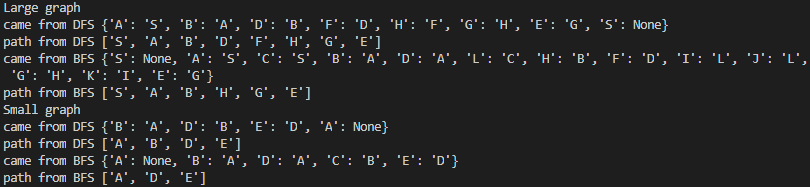
\includegraphics[scale=0.6]{BFSvsDFS.png}}
\vspace{3mm}
\subsubsection{UniformCostSearch}
\centerline{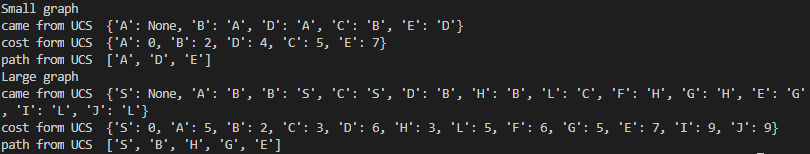
\includegraphics[scale=0.6]{UCS.png}}
\vspace{3mm}
\subsubsection{AStarSearch}
\centerline{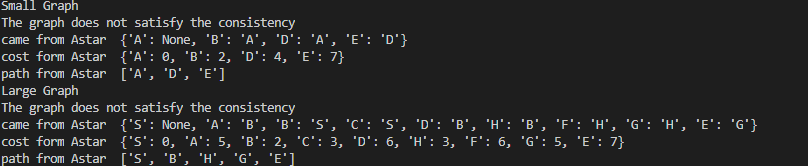
\includegraphics[scale=0.6]{A_star.png}}
\vspace{3mm}
\subsection{Extra credit}
\subsubsection{Valid node}
To check whether the goal and start state are valid nodes in the graph, I think there are two points we need to detect.
\begin{enumerate}
\item
Detect whether the start node and goal node are in the graph\\
The best way to detect this point, we can define some method objects in the class \emph{Graph}.
In this way, every time the algorithm want to get imformation such 
as node's edges and location, we can detect whether the node is in the 
graph. If not, print ``The node is not in the graph''\\
\item
Detect whether there's a way from the start to the goal node.\\
If the algorithm has traversaed all the nodes and edges but still doesn't find a path,
the node won't in dictionay \emph{came\_from}'s keys. So if the \emph{came\_from[goal]} 
goes wrong, print ``There's no path from start to goal''.
\end{enumerate}
\subsubsection{Check consistency}
To check the graph satisfies the consistency of heuristics, we need to define a method object \\
\emph{checkConsistency} in class \emph{Graph}.
Once we want to check a graph's consistency, we just use code\\ \emph{Graph.checkConsistency(goal)}\\
\centerline{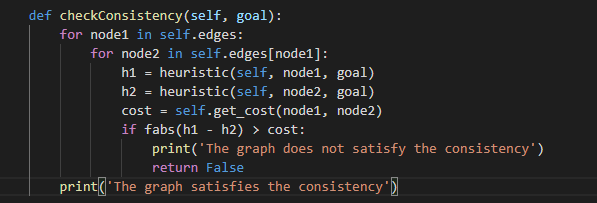
\includegraphics[scale=0.8]{Check.png}}\\
\end{document}